\chapter{EARLY INVESTIGATION: HARDWARE ABSTRACTION}
\label{hardware}
Initial research into the domain of SDN was based around the utilization
of frameworks providing low level access to networking resources. In order
to maintain high performance in user level application space, these devices
need to be abstracted. Network interfaces, both logical and physical, can
expose a variety of capabilities and features that need to be encapsulated
to improve portability and optimal usage. The same is true for computational
devices, including CPUs, Network Processing Units (NPUs), and other various
hardware accelerators. This chapter discusses the evaluation of low level
port abstractions provided by DPDK, Section \ref{hardware:dpdk}, and Netmap,
Section \ref{hardware:netmap}, mid-level port abstractions implemented in ODP,
Section \ref{hardware:odp}, as well as the conclusions drawn in Section
\ref{hardware:concl}.

\section{DPDK}
\label{hardware:dpdk}
Intel's DPDK provides users with a framework on which data plane applications
can be built utilizing highly optimized constructs and device drivers. At the
time of this investigation, the project was in the early stages of development
(version 1.0, 1.1). The drivers provided by the development kit are written
specifically for Intel brand networking devices. Systems that lack compatible
hardware can provision a virtual machine to take advantage of the optimized
port drivers available. In order to execute an application with the DPDK runtime
environment, the host operating system requires some additional modifications
as well. A custom networking kernel module allows applications to bypass the
host systems native networking stack, reducing the number of copies made
between user and kernel space. Memory page size is also increased to reduce
the number of page faults.

\begin{figure}[h]
  \centering
  \begin{subfigure}[b]{0.48\textwidth}
    \centering
    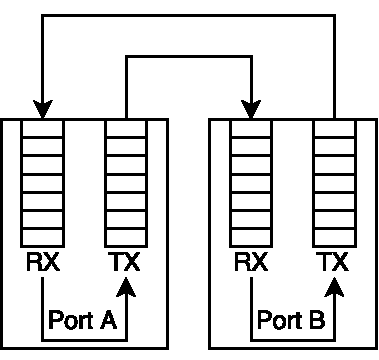
\includegraphics{dpdk_l2_a}
    \caption{DPDK provided forwarding behavior, where a pair of ports sends
    data to and receives from the other.}
  \end{subfigure}
  \hfill
  \begin{subfigure}[b]{0.48\textwidth}
    \centering
    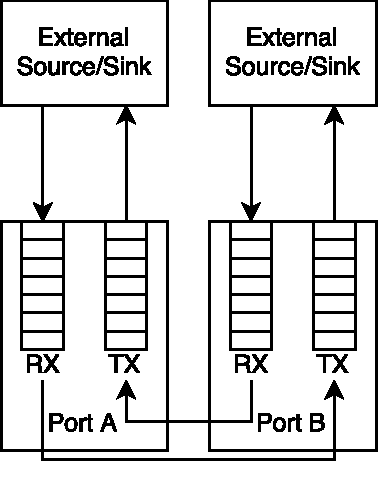
\includegraphics{dpdk_l2_b}
    \caption{Modified forwarding behavior, where a pair of ports sends the data
    received by the other.}
  \end{subfigure}
  \caption{DPDK L2 forwarding models.}
  \label{dpdk_l2}
\end{figure}

The goal of the experiment is to create a virtual ``wire'' between two Ethernet
ports, such that data recieved by port A is sent by port B, and vice versa. An
example application, L2 Forward, provided in the development kit served as a
starting point for this experiment. The example creates an \emph{external}
wire between pairs of ports, where port A sends data to port B, and B sends to
A. In order to create an \emph{internal} wire, the driver for each port needed
to be changed. Figure \ref{dpdk_l2} illustrates the behavior models used in the
experiment. The modified implementation has each port reads from it's
counterparts receive queue and sends a copy from itself.  The destination
address fields have to be refactored from being statically hard coded in the
port driver to a dynamic, mutable property.

\begin{figure}[h]
  \centering
  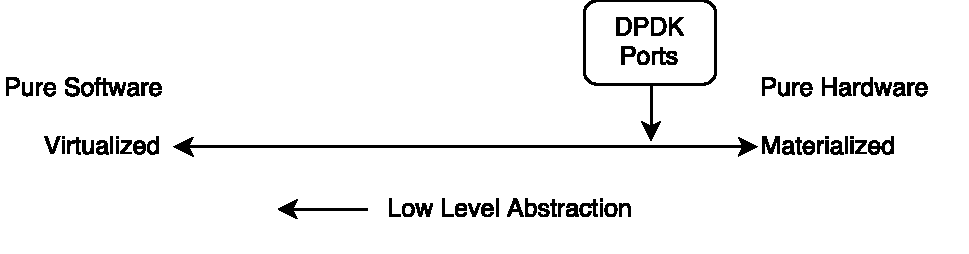
\includegraphics[scale=0.75]{spectrum_dpdk}
  \caption{DPDK's port abstraction limits portability by being too hardware
  specific.}
  \label{hardware:spectrum_dpdk}
\end{figure}

Execution of the modified application gives inconsistent results, and can
require system restarts between runs to reconfigure the virtual machine when
errors occur. This is attributed to performance and abstraction penalties
suffered from the use of the virtual machine as the runtime environment host.
Though DPDK's optimized port drivers deliver solid performance,
The results show that utilizing this framework for abstracting low level port
resources would narrow the field of compatible physical devices to target.

\section{Netmap}
\label{hardware:netmap}
The second framework evaluated for port abstraction comes from the netmap
project. Netmap provides low level access to network interfaces by diverting
the flow of data to and from the interface away from the operating system, and
towards a custom device.

\begin{figure}[h]
  \centering
  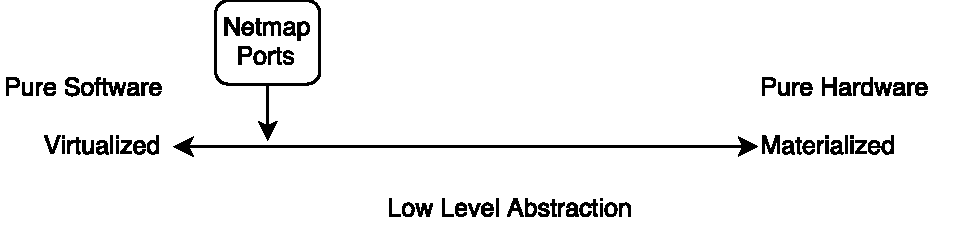
\includegraphics[scale=0.75]{spectrum_netmap}
  \caption{Netmap's port abstraction is more portable, but incurs performance
  penalties.}
  \label{hardware:spectrum_netmap}
\end{figure}

Blah blah blah.

\section{ODP}
\label{hardware:odp}
Stuff on ODP.

\begin{figure}[h]
  \centering
  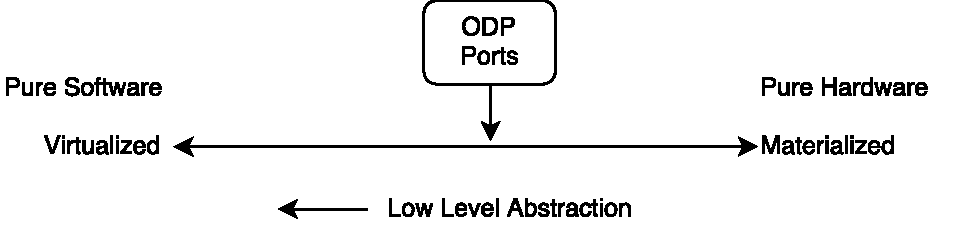
\includegraphics[scale=0.75]{spectrum_odp}
  \caption{ODP's port abstraction strikes a good balance between portability
  and performance, and is currently being considered.}
  \label{hardware:spectrum_odp}
\end{figure}

\section{Conclusions}
\label{hardware:concl}
Stuff was done.
